\documentclass[a4paper,12pt]{article}

\usepackage[utf8x]{inputenc}
\usepackage[T2A]{fontenc}
\usepackage[english, russian]{babel}

% Опционно, требует  apt-get install scalable-cyrfonts.*
% и удаления одной строчки в cyrtimes.sty
% Сточку не удалять!
% \usepackage{cyrtimes}

% Картнки и tikz
\usepackage{graphicx}
\usepackage{tikz}
\usetikzlibrary{snakes,arrows,shapes}


% Некоторая русификация.
\usepackage{misccorr}
\usepackage{indentfirst}
\renewcommand{\labelitemi}{\normalfont\bfseries{--}}

% Увы, поля придётся уменьшить из-за листингов.
\topmargin -1cm
\oddsidemargin -0.5cm
\evensidemargin -0.5cm
\textwidth 17cm
\textheight 24cm

\sloppy

% Оглавление в PDF
\usepackage[
bookmarks=true,
colorlinks=true, linkcolor=black, anchorcolor=black, citecolor=black, menucolor=black,filecolor=black, urlcolor=black,
unicode=true
]{hyperref}

% Для исходного кода в тексте
\newcommand{\Code}[1]{\texttt{#1}}


\title{Отчёт по лабораторной работе \\ <<IP-маршрутизация>>}
\author{Здесь Ф.~И.~О}

\begin{document}

\maketitle

\tableofcontents

% Текст отчёта должен быть читаемым!!! Написанное здесь является рыбой.

\section{Топология сети}

Топология сети и используемые IP-адреса показаны на рис.~\ref{fig:network}.

\begin{figure}
\centering
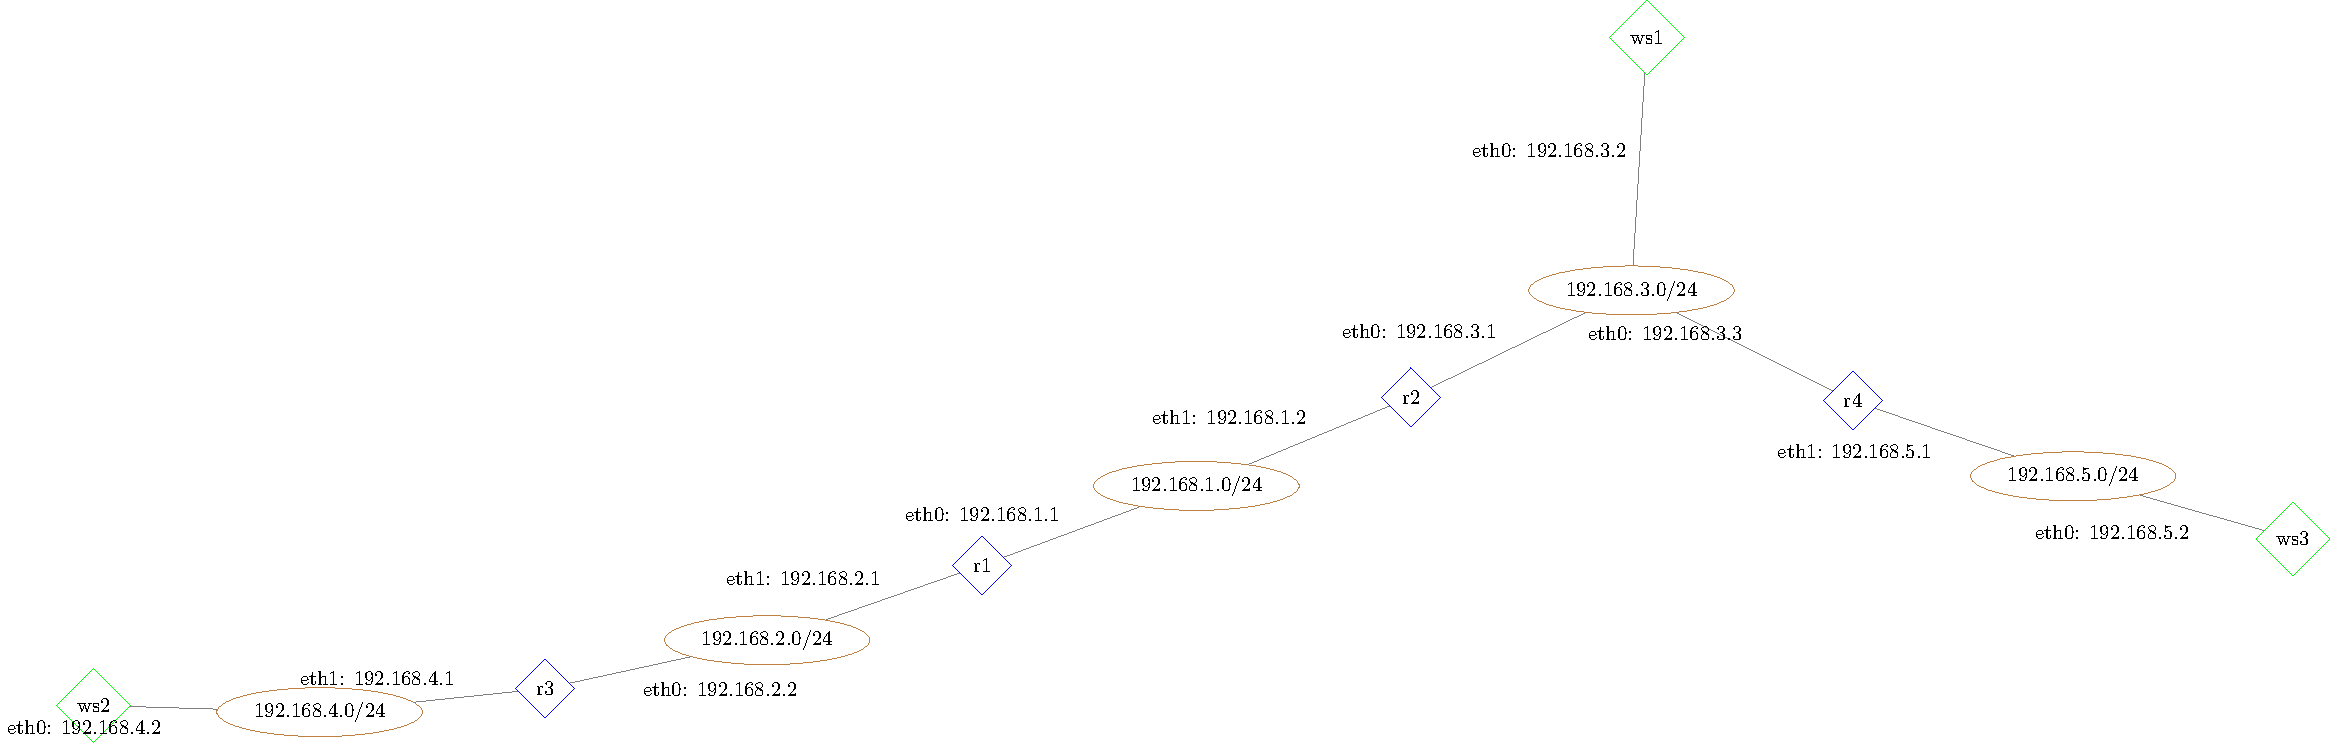
\includegraphics[width=\textwidth]{includes/network_gv.pdf}
\caption{Топология сети}
\label{fig:network}
\end{figure}
\newpage

\section{Назначение IP-адресов}
Ниже приведён файл настройки протокола IP маршрутизатора r1.

\begin{Verbatim}
auto lo
iface lo inet loopback

auto eth0
iface eth0 inet static
    address 192.168.1.1
    netmask 255.255.255.0
    up ip r add 192.168.3.0/24 via 192.168.1.2 dev eth0
    down ip r del 192.168.3.0/24
    up ip r add 192.168.5.0/24 via 192.168.1.2 dev eth0
    down ip r del 192.168.5.0/24
    
auto eth1
iface eth1 inet static
    address 192.168.2.1
    netmask 255.255.255.0
    up ip r add 192.168.4.0/24 via 192.168.2.2 dev eth1
    down ip r del 192.168.4.0/24
\end{Verbatim}

Ниже приведён файл настройки протокола IP маршрутизатора r2.

\begin{Verbatim}
auto lo
iface lo inet loopback

auto eth0
iface eth0 inet static
    address 192.168.3.1
    netmask 255.255.255.0
    up ip r add 192.168.5.0/24 via 192.168.3.3 dev eth0
    down ip r del 192.168.5.0/24

auto eth1
iface eth1 inet static
    address 192.168.1.2
    netmask 255.255.255.0
    up ip r add 192.168.2.0/24 via 192.168.1.1 dev eth1
    down ip r del 192.168.2.0/24
    up ip r add 192.168.4.0/24 via 192.168.1.1 dev eth1
    down ip r del 192.168.4.0/24
\end{Verbatim}

Ниже приведён файл настройки протокола IP маршрутизатора r3.

\begin{Verbatim}
auto lo
iface lo inet loopback

auto eth0
iface eth0 inet static
    address 192.168.2.2
    netmask 255.255.255.0
    up ip r add 192.168.1.0/24 via 192.168.2.1 dev eth0
    down ip r del 192.168.1.0/24
    up ip r add 192.168.3.0/24 via 192.168.2.1 dev eth0
    down ip r del 192.168.3.0/24
    up ip r add 192.168.5.0/24 via 192.168.2.1 dev eth0
    down ip r del 192.168.5.0/24

auto eth1
iface eth1 inet static
    address 192.168.4.1
    netmask 255.255.255.0
\end{Verbatim}

Ниже приведён файл настройки протокола IP маршрутизатора r4.

\begin{Verbatim}
auto lo
iface lo inet loopback

auto eth0
iface eth0 inet static
    address 192.168.3.3
    netmask 255.255.255.0
    up ip r add 192.168.1.0/24 via 192.168.3.1 dev eth0
    down ip r del 192.168.1.0/24
    up ip r add 192.168.2.0/24 via 192.168.3.1 dev eth0
    down ip r del 192.168.2.0/24
    up ip r add 192.168.4.0/24 via 192.168.3.1 dev eth0
    down ip r del 192.168.4.0/24

auto eth1
iface eth1 inet static
    address 192.168.5.1
    netmask 255.255.255.0
\end{Verbatim}



Ниже приведён файл настройки протокола IP рабочей станции ws1.

\begin{Verbatim}
auto lo
iface lo inet loopback

auto eth0
iface eth0 inet static
	address 192.168.3.2
	netmask 255.255.255.0
	up ip r add 192.168.1.0/24 via 192.168.3.1 dev eth0
    down ip r del 192.168.1.0/24
	up ip r add 192.168.5.0/24 via 192.168.3.3 dev eth0
    down ip r del 192.168.5.0/24
	up ip r add 192.168.2.0/24 via 192.168.3.1 dev eth0
    down ip r del 192.168.2.0/24
	up ip r add 192.168.4.0/24 via 192.168.3.1 dev eth0
    down ip r del 192.168.4.0/24
\end{Verbatim}


Ниже приведён файл настройки протокола IP рабочей станции ws2.

\begin{Verbatim}
auto lo
iface lo inet loopback

auto eth0
iface eth0 inet static
    address 192.168.4.2
    netmask 255.255.255.0
    gateway 192.168.4.1
\end{Verbatim}

Ниже приведён файл настройки протокола IP рабочей станции ws3.

\begin{Verbatim}
auto lo
iface lo inet loopback

auto eth0
iface eth0 inet static
    address 192.168.5.2
    netmask 255.255.255.0
    gateway 192.168.5.1
\end{Verbatim}



\section{Таблица маршрутизации}

Таблица маршрутизации для \textbf{r1}.

\begin{Verbatim}
192.168.5.0/24 via 192.168.1.2 dev eth0 
192.168.4.0/24 via 192.168.2.2 dev eth1 
192.168.3.0/24 via 192.168.1.2 dev eth0 
192.168.2.0/24 dev eth1  proto kernel  scope link  src 192.168.2.1 
192.168.1.0/24 dev eth0  proto kernel  scope link  src 192.168.1.1
\end{Verbatim}

Таблица маршрутизации для \textbf{r2}.

\begin{Verbatim}
192.168.5.0/24 via 192.168.3.3 dev eth0 
192.168.4.0/24 via 192.168.1.1 dev eth1 
192.168.3.0/24 dev eth0  proto kernel  scope link  src 192.168.3.1 
192.168.2.0/24 via 192.168.1.1 dev eth1 
192.168.1.0/24 dev eth1  proto kernel  scope link  src 192.168.1.2
\end{Verbatim}

Таблица маршрутизации для \textbf{r3}.

\begin{Verbatim}
192.168.5.0/24 via 192.168.2.1 dev eth0 
192.168.4.0/24 dev eth1  proto kernel  scope link  src 192.168.4.1 
192.168.3.0/24 via 192.168.2.1 dev eth0 
192.168.2.0/24 dev eth0  proto kernel  scope link  src 192.168.2.2 
192.168.1.0/24 via 192.168.2.1 dev eth0
\end{Verbatim}

Таблица маршрутизации для \textbf{r4}.

\begin{Verbatim}
192.168.5.0/24 dev eth1  proto kernel  scope link  src 192.168.5.1 
192.168.4.0/24 via 192.168.3.1 dev eth0 
192.168.3.0/24 dev eth0  proto kernel  scope link  src 192.168.3.3 
192.168.2.0/24 via 192.168.3.1 dev eth0 
192.168.1.0/24 via 192.168.3.1 dev eth0
\end{Verbatim}


Таблица маршрутизации для \textbf{ws1}.

\begin{Verbatim}
192.168.5.0/24 via 192.168.3.3 dev eth0 
192.168.4.0/24 via 192.168.3.1 dev eth0 
192.168.3.0/24 dev eth0  proto kernel  scope link  src 192.168.3.2 
192.168.2.0/24 via 192.168.3.1 dev eth0 
192.168.1.0/24 via 192.168.3.1 dev eth0
\end{Verbatim}



% ... Повторять для всех маршрутизаторов и рабочих станций, где есть что-то кроме gateway.

\section{Проверка настройки сети}

Вывод \textbf{traceroute} от узла ws1 до ws2 при нормальной работе сети.

\begin{Verbatim}
traceroute to 192.168.4.2 (192.168.4.2), 64 hops max, 40 byte packets
 1  192.168.3.1 (192.168.3.1)  0 ms  0 ms  0 ms
 2  192.168.1.1 (192.168.1.1)  0 ms  0 ms  0 ms
 3  192.168.2.2 (192.168.2.2)  0 ms  0 ms  0 ms
 4  192.168.4.2 (192.168.4.2)  1 ms  0 ms  0 ms
\end{Verbatim}

Вывод \textbf{traceroute} от узла ws1 до ws3 при нормальной работе сети.

\begin{Verbatim}
traceroute to 192.168.5.2 (192.168.5.2), 64 hops max, 40 byte packets
 1  192.168.3.3 (192.168.3.3)  9 ms  0 ms  0 ms
 2  192.168.5.2 (192.168.5.2)  12 ms  1 ms  1 ms
\end{Verbatim}

Вывод \textbf{traceroute} от узла ws2 до ws3 при нормальной работе сети.

\begin{Verbatim}
traceroute to 192.168.5.2 (192.168.5.2), 64 hops max, 40 byte packets
 1  192.168.4.1 (192.168.4.1)  1 ms  2 ms  1 ms
 2  192.168.2.1 (192.168.2.1)  1 ms  1 ms  1 ms
 3  192.168.1.2 (192.168.1.2)  2 ms  2 ms  2 ms
 4  192.168.3.3 (192.168.3.3)  13 ms  2 ms  2 ms
 5  192.168.5.2 (192.168.5.2)  2 ms  2 ms  2 ms
\end{Verbatim}

Вывод \textbf{traceroute} от узла ws2 до ws1 при нормальной работе сети.

\begin{Verbatim}
traceroute to 192.168.3.2 (192.168.3.2), 64 hops max, 40 byte packets
 1  192.168.4.1 (192.168.4.1)  0 ms  0 ms  0 ms
 2  192.168.2.1 (192.168.2.1)  0 ms  0 ms  1 ms
 3  192.168.1.2 (192.168.1.2)  1 ms  1 ms  1 ms
 4  192.168.3.2 (192.168.3.2)  1 ms  1 ms  1 ms
\end{Verbatim}

Вывод \textbf{traceroute} от узла ws3 до ws1 при нормальной работе сети.

\begin{Verbatim}
traceroute to 192.168.3.2 (192.168.3.2), 64 hops max, 40 byte packets
 1  192.168.5.1 (192.168.5.1)  1 ms  1 ms  1 ms
 2  192.168.3.2 (192.168.3.2)  1 ms  1 ms  1 ms
\end{Verbatim}
Вывод \textbf{traceroute} от узла ws3 до ws2 при нормальной работе сети.

\begin{Verbatim}
traceroute to 192.168.4.2 (192.168.4.2), 64 hops max, 40 byte packets
 1  192.168.5.1 (192.168.5.1)  1 ms  1 ms  0 ms
 2  192.168.3.1 (192.168.3.1)  0 ms  0 ms  0 ms
 3  192.168.1.1 (192.168.1.1)  1 ms  1 ms  0 ms
 4  192.168.2.2 (192.168.2.2)  1 ms  1 ms  1 ms
 5  192.168.4.2 (192.168.4.2)  1 ms  1 ms  1 ms
\end{Verbatim}

Перехват трафика на r1, вызвана команда traceroute 192.168.5.2 на машине ws2
\begin{Verbatim}
07:48:10.904898 ee:97:f2:ab:47:0c > ff:ff:ff:ff:ff:ff, ethertype ARP (0x0806), length 42: arp who-has 192.168.2.1 tell 192.168.2.2
07:48:10.904979 fa:de:dc:30:96:57 > ee:97:f2:ab:47:0c, ethertype ARP (0x0806), length 42: arp reply 192.168.2.1 is-at fa:de:dc:30:96:57
07:48:10.905388 ee:97:f2:ab:47:0c > fa:de:dc:30:96:57, ethertype IPv4 (0x0800), length 54: (tos 0x0, ttl 1, id 32087, offset 0, flags [none], proto UDP (17), length 40) 192.168.4.2.33323 > 192.168.5.2.33438: UDP, length 12
07:48:10.905470 fa:de:dc:30:96:57 > ee:97:f2:ab:47:0c, ethertype IPv4 (0x0800), length 82: (tos 0xc0, ttl 64, id 3491, offset 0, flags [none], proto ICMP (1), length 68) 192.168.2.1 > 192.168.4.2: ICMP time exceeded in-transit, length 48
	(tos 0x0, ttl 1, id 32087, offset 0, flags [none], proto UDP (17), length 40) 192.168.4.2.33323 > 192.168.5.2.33438: UDP, length 12
07:48:10.908365 ee:97:f2:ab:47:0c > fa:de:dc:30:96:57, ethertype IPv4 (0x0800), length 54: (tos 0x0, ttl 1, id 32088, offset 0, flags [none], proto UDP (17), length 40) 192.168.4.2.33323 > 192.168.5.2.33439: UDP, length 12
07:48:10.908389 fa:de:dc:30:96:57 > ee:97:f2:ab:47:0c, ethertype IPv4 (0x0800), length 82: (tos 0xc0, ttl 64, id 3492, offset 0, flags [none], proto ICMP (1), length 68) 192.168.2.1 > 192.168.4.2: ICMP time exceeded in-transit, length 48
	(tos 0x0, ttl 1, id 32088, offset 0, flags [none], proto UDP (17), length 40) 192.168.4.2.33323 > 192.168.5.2.33439: UDP, length 12
07:48:10.909388 ee:97:f2:ab:47:0c > fa:de:dc:30:96:57, ethertype IPv4 (0x0800), length 54: (tos 0x0, ttl 1, id 32089, offset 0, flags [none], proto UDP (17), length 40) 192.168.4.2.33323 > 192.168.5.2.33440: UDP, length 12
07:48:10.909411 fa:de:dc:30:96:57 > ee:97:f2:ab:47:0c, ethertype IPv4 (0x0800), length 82: (tos 0xc0, ttl 64, id 3493, offset 0, flags [none], proto ICMP (1), length 68) 192.168.2.1 > 192.168.4.2: ICMP time exceeded in-transit, length 48
	(tos 0x0, ttl 1, id 32089, offset 0, flags [none], proto UDP (17), length 40) 192.168.4.2.33323 > 192.168.5.2.33440: UDP, length 12
07:48:10.910453 ee:97:f2:ab:47:0c > fa:de:dc:30:96:57, ethertype IPv4 (0x0800), length 54: (tos 0x0, ttl 2, id 32090, offset 0, flags [none], proto UDP (17), length 40) 192.168.4.2.33323 > 192.168.5.2.33441: UDP, length 12
07:48:10.922329 fa:de:dc:30:96:57 > ee:97:f2:ab:47:0c, ethertype IPv4 (0x0800), length 82: (tos 0xc0, ttl 63, id 54534, offset 0, flags [none], proto ICMP (1), length 68) 192.168.1.2 > 192.168.4.2: ICMP time exceeded in-transit, length 48
	(tos 0x0, ttl 1, id 32090, offset 0, flags [none], proto UDP (17), length 40) 192.168.4.2.33323 > 192.168.5.2.33441: UDP, length 12
07:48:10.925538 ee:97:f2:ab:47:0c > fa:de:dc:30:96:57, ethertype IPv4 (0x0800), length 54: (tos 0x0, ttl 2, id 32091, offset 0, flags [none], proto UDP (17), length 40) 192.168.4.2.33323 > 192.168.5.2.33442: UDP, length 12
07:48:10.925880 fa:de:dc:30:96:57 > ee:97:f2:ab:47:0c, ethertype IPv4 (0x0800), length 82: (tos 0xc0, ttl 63, id 54535, offset 0, flags [none], proto ICMP (1), length 68) 192.168.1.2 > 192.168.4.2: ICMP time exceeded in-transit, length 48
	(tos 0x0, ttl 1, id 32091, offset 0, flags [none], proto UDP (17), length 40) 192.168.4.2.33323 > 192.168.5.2.33442: UDP, length 12
07:48:10.926996 ee:97:f2:ab:47:0c > fa:de:dc:30:96:57, ethertype IPv4 (0x0800), length 54: (tos 0x0, ttl 2, id 32092, offset 0, flags [none], proto UDP (17), length 40) 192.168.4.2.33323 > 192.168.5.2.33443: UDP, length 12
07:48:10.927295 fa:de:dc:30:96:57 > ee:97:f2:ab:47:0c, ethertype IPv4 (0x0800), length 82: (tos 0xc0, ttl 63, id 54536, offset 0, flags [none], proto ICMP (1), length 68) 192.168.1.2 > 192.168.4.2: ICMP time exceeded in-transit, length 48
	(tos 0x0, ttl 1, id 32092, offset 0, flags [none], proto UDP (17), length 40) 192.168.4.2.33323 > 192.168.5.2.33443: UDP, length 12
07:48:10.928550 ee:97:f2:ab:47:0c > fa:de:dc:30:96:57, ethertype IPv4 (0x0800), length 54: (tos 0x0, ttl 3, id 32093, offset 0, flags [none], proto UDP (17), length 40) 192.168.4.2.33323 > 192.168.5.2.33444: UDP, length 12
07:48:10.940202 fa:de:dc:30:96:57 > ee:97:f2:ab:47:0c, ethertype IPv4 (0x0800), length 82: (tos 0xc0, ttl 62, id 1547, offset 0, flags [none], proto ICMP (1), length 68) 192.168.3.3 > 192.168.4.2: ICMP time exceeded in-transit, length 48
	(tos 0x0, ttl 1, id 32093, offset 0, flags [none], proto UDP (17), length 40) 192.168.4.2.33323 > 192.168.5.2.33444: UDP, length 12
07:48:10.944583 ee:97:f2:ab:47:0c > fa:de:dc:30:96:57, ethertype IPv4 (0x0800), length 54: (tos 0x0, ttl 3, id 32094, offset 0, flags [none], proto UDP (17), length 40) 192.168.4.2.33323 > 192.168.5.2.33445: UDP, length 12
07:48:10.945622 fa:de:dc:30:96:57 > ee:97:f2:ab:47:0c, ethertype IPv4 (0x0800), length 82: (tos 0xc0, ttl 62, id 1548, offset 0, flags [none], proto ICMP (1), length 68) 192.168.3.3 > 192.168.4.2: ICMP time exceeded in-transit, length 48
	(tos 0x0, ttl 1, id 32094, offset 0, flags [none], proto UDP (17), length 40) 192.168.4.2.33323 > 192.168.5.2.33445: UDP, length 12
07:48:10.947072 ee:97:f2:ab:47:0c > fa:de:dc:30:96:57, ethertype IPv4 (0x0800), length 54: (tos 0x0, ttl 3, id 32095, offset 0, flags [none], proto UDP (17), length 40) 192.168.4.2.33323 > 192.168.5.2.33446: UDP, length 12
07:48:10.948094 fa:de:dc:30:96:57 > ee:97:f2:ab:47:0c, ethertype IPv4 (0x0800), length 82: (tos 0xc0, ttl 62, id 1549, offset 0, flags [none], proto ICMP (1), length 68) 192.168.3.3 > 192.168.4.2: ICMP time exceeded in-transit, length 48
	(tos 0x0, ttl 1, id 32095, offset 0, flags [none], proto UDP (17), length 40) 192.168.4.2.33323 > 192.168.5.2.33446: UDP, length 12
07:48:10.949714 ee:97:f2:ab:47:0c > fa:de:dc:30:96:57, ethertype IPv4 (0x0800), length 54: (tos 0x0, ttl 4, id 32096, offset 0, flags [none], proto UDP (17), length 40) 192.168.4.2.33323 > 192.168.5.2.33447: UDP, length 12
07:48:10.961675 fa:de:dc:30:96:57 > ee:97:f2:ab:47:0c, ethertype IPv4 (0x0800), length 82: (tos 0xc0, ttl 61, id 40025, offset 0, flags [none], proto ICMP (1), length 68) 192.168.5.2 > 192.168.4.2: ICMP 192.168.5.2 udp port 33447 unreachable, length 48
	(tos 0x0, ttl 1, id 32096, offset 0, flags [none], proto UDP (17), length 40) 192.168.4.2.33323 > 192.168.5.2.33447: UDP, length 12
07:48:10.965966 ee:97:f2:ab:47:0c > fa:de:dc:30:96:57, ethertype IPv4 (0x0800), length 54: (tos 0x0, ttl 4, id 32097, offset 0, flags [none], proto UDP (17), length 40) 192.168.4.2.33323 > 192.168.5.2.33448: UDP, length 12
07:48:10.967025 fa:de:dc:30:96:57 > ee:97:f2:ab:47:0c, ethertype IPv4 (0x0800), length 82: (tos 0xc0, ttl 61, id 40026, offset 0, flags [none], proto ICMP (1), length 68) 192.168.5.2 > 192.168.4.2: ICMP 192.168.5.2 udp port 33448 unreachable, length 48
	(tos 0x0, ttl 1, id 32097, offset 0, flags [none], proto UDP (17), length 40) 192.168.4.2.33323 > 192.168.5.2.33448: UDP, length 12
07:48:10.968620 ee:97:f2:ab:47:0c > fa:de:dc:30:96:57, ethertype IPv4 (0x0800), length 54: (tos 0x0, ttl 4, id 32098, offset 0, flags [none], proto UDP (17), length 40) 192.168.4.2.33323 > 192.168.5.2.33449: UDP, length 12
07:48:10.969990 fa:de:dc:30:96:57 > ee:97:f2:ab:47:0c, ethertype IPv4 (0x0800), length 82: (tos 0xc0, ttl 61, id 40027, offset 0, flags [none], proto ICMP (1), length 68) 192.168.5.2 > 192.168.4.2: ICMP 192.168.5.2 udp port 33449 unreachable, length 48
	(tos 0x0, ttl 1, id 32098, offset 0, flags [none], proto UDP (17), length 40) 192.168.4.2.33323 > 192.168.5.2.33449: UDP, length 12
07:48:15.898234 fa:de:dc:30:96:57 > ee:97:f2:ab:47:0c, ethertype ARP (0x0806), length 42: arp who-has 192.168.2.2 tell 192.168.2.1
07:48:15.898815 ee:97:f2:ab:47:0c > fa:de:dc:30:96:57, ethertype ARP (0x0806), length 42: arp reply 192.168.2.2 is-at ee:97:f2:ab:47:0c
\end{Verbatim}


\section{Маршрутизация}

% На пути здесь достаточно быть одному маршрутизатору!

MAC адреса интерфейсов в опыте:
\begin{Verbatim}
ws1 eth0(192.168.3.2/24) - a6:f9:52:b6:1e:69
r4 eth0(192.168.3.3/24) - 4a:e4:d9:3b:f2:04
r4 eth1(192.168.5.1/24) - 42:9b:97:db:b0:a6
ws3 eth0(192.168.5.2/24) - b2:0b:69:d6:a7:1e
\end{Verbatim}


Таблица маршрутизатора r4:
\begin{Verbatim}
192.168.5.0/24 dev eth1  proto kernel  scope link  src 192.168.5.1 
192.168.4.0/24 via 192.168.3.1 dev eth0 
192.168.3.0/24 dev eth0  proto kernel  scope link  src 192.168.3.3 
192.168.2.0/24 via 192.168.3.1 dev eth0 
192.168.1.0/24 via 192.168.3.1 dev eth0 
\end{Verbatim}

Показаны опыты после стирания кеша ARP.
% Не забудьте это сделать!
Далее показана отправка пакета на маршрутизатор (косвенная маршрутизация). 

\begin{Verbatim}
a6:f9:52:b6:1e:69 > ff:ff:ff:ff:ff:ff, ethertype ARP (0x0806), \\ 
length 42: arp who-has 192.168.3.3 tell 192.168.3.2 \\
\\
4a:e4:d9:3b:f2:04 > a6:f9:52:b6:1e:69, ethertype ARP (0x0806), \\ 
length 42: arp reply 192.168.3.3 is-at 4a:e4:d9:3b:f2:04 \\
\\
a6:f9:52:b6:1e:69 > 4a:e4:d9:3b:f2:04, ethertype IPv4 (0x0800), \\ 
length 98: 192.168.3.2 > 192.168.5.2: \\
ICMP echo request, id 22786, seq 1, length 64
\end{Verbatim}

Затем маршрутизатор отправил его далее.

\begin{Verbatim}
42:9b:97:db:b0:a6 > ff:ff:ff:ff:ff:ff, ethertype ARP (0x0806), \\
length 42: arp who-has 192.168.5.2 tell 192.168.5.1 \\
\\
b2:0b:69:d6:a7:1e > 42:9b:97:db:b0:a6, ethertype ARP (0x0806), \\ 
length 42: arp reply 192.168.5.2 is-at b2:0b:69:d6:a7:1e \\
\\
42:9b:97:db:b0:a6 > b2:0b:69:d6:a7:1e, ethertype IPv4 (0x0800), \\ 
length 98: 192.168.3.2 > 192.168.5.2: \\
ICMP echo request, id 22786, seq 1, length 64
\end{Verbatim}

\section{Продолжительность жизни пакета}

MAC адреса интерфейсов в опыте:
\begin{Verbatim}
r3 eth0(192.168.2.2/24) - ee:97:f2:ab:47:0c
r1 eth1(192.168.2.1/24) - fa:de:dc:30:96:57
\end{Verbatim}

Создал петлю на маршрутизаторе r1, отключив на нем интерфейс eth0 и добавив неверный маршрут до сети 192.168.5.0/24 для этого выполнил следующие команды: 
\begin{Verbatim}
ip link set eth0 down
ip route add 192.168.5.0/24 via 192.168.2.2 dev eth1
\end{Verbatim}

Измененная таблица маршрутизации на маршрутизаторе r1:
\begin{Verbatim}
192.168.5.0/24 via 192.168.2.2 dev eth1 
192.168.4.0/24 via 192.168.2.2 dev eth1 
192.168.2.0/24 dev eth1  proto kernel  scope link  src 192.168.2.1
\end{Verbatim}

Запустил программу перехвата сетевого трафика на маршрутизаторе r1 (tcpdump -tnve -i eth1) и r3 (tcpdump -tnve -i eth0). Послал эхо-запрос из машины ws2(192.168.4.2) на машину ws3(192.168.5.2) в сети 192.168.5.0/24.
\begin{Verbatim}
ping -c 1 192.168.5.2
\end{Verbatim}

Результат:

\begin{Verbatim}
fa:de:dc:30:96:57 > ee:97:f2:ab:47:0c, ethertype IPv4 (0x0800), length 98: (tos 0x0, ttl 2, \\ 
id 0, offset 0, flags [DF], proto ICMP (1), length 84) 192.168.4.2 > 192.168.5.2: \\
ICMP echo request, id 18434, seq 1, length 64 \\
\\
ee:97:f2:ab:47:0c > fa:de:dc:30:96:57, ethertype IPv4 (0x0800), length 98: (tos 0x0, ttl 1, \\ 
id 0, offset 0, flags [DF], proto ICMP (1), length 84) 192.168.4.2 > 192.168.5.2: \\
ICMP echo request, id 18434, seq 1, length 64 \\
\\
fa:de:dc:30:96:57 > ee:97:f2:ab:47:0c, ethertype IPv4 (0x0800), length 126: (tos 0xc0, ttl 64, \\
id 2480, offset 0, flags [none], proto ICMP (1), length 112) 192.168.2.1 > 192.168.4.2: \\
ICMP time exceeded in-transit, length 92
\end{Verbatim}

Сообщение о завершении жизни отправил маршрутизатор r1
\section{Изучение IP-фрагментации}

Изменил значение MTU для сети 192.168.2.0/24, для этого выполнил на маршрутизаторе r1 команду:
\begin{Verbatim}
ip link set dev eth1 mtu 576
\end{Verbatim}
также выполнил на маршрутизаторе r3 команду: 
\begin{Verbatim}
ip link set dev eth0 mtu 576
\end{Verbatim}

% Напоминаем, что PMTU следует отключить!

На машине ws2 отключил флаг DF (механизм борьбы с фрагментацией):
\begin{Verbatim}
echo 1 > /proc/sys/net/ipv4/ip_no_pmtu_disc
\end{Verbatim}
Затем послал эхо запрос с этой машины на маршрутизатор r2(192.168.3.1)
\begin{Verbatim}
ping -c 1 -s 1000 192.168.3.1
\end{Verbatim}


Вывод \textbf{tcpdump} на маршрутизаторе r3 перед сетью с уменьшенным MTU.

% Вывод в ширину можно и сократить, удалив несущественные моменты!

\begin{Verbatim}
IP (... offset 0, flags [none], proto ICMP (1), length 1028) 192.168.4.2 > 192.168.3.1: ...
IP (... offset 0, flags [none], proto ICMP (1), length 1028) 192.168.3.1 > 192.168.4.2: ...
\end{Verbatim}

Вывод \textbf{tcpdump} на маршрутизаторе r1 после сети с уменьшенным MTU.

% Вывод в ширину можно и сократить, удалив несущественные моменты!

\begin{Verbatim}
IP (... offset 0, flags [+], proto ICMP (1), length 572) 192.168.4.2 > 192.168.3.1: ...
IP (... offset 552, flags [none], proto ICMP (1), length 476) 192.168.4.2 > 192.168.3.1: icmp
IP (... offset 0, flags [+], proto ICMP (1), length 572) 192.168.3.1 > 192.168.4.2: ...
IP (... offset 552, flags [none], proto ICMP (1), length 476) 192.168.3.1 > 192.168.4.2: icmp
\end{Verbatim}


Вывод \textbf{tcpdump} на узле получателя r2.

\begin{Verbatim}
IP (... offset 0, flags [none], proto ICMP (1), length 1028) 192.168.4.2 > 192.168.3.1: ...
IP (... offset 0, flags [none], proto ICMP (1), length 1028) 192.168.3.1 > 192.168.4.2: ...
\end{Verbatim}


\section{Отсутствие сети}

Запустил на маршрутизаторе r3 перехват сетевого трафика с помощью команды: 
\begin{Verbatim}
tcpdump -n -i eth1 icmp
\end{Verbatim}

На машине ws2 выполнил эхо запрос к несуществующей сети: 
\begin{Verbatim}
ping -c 1 10.30.0.111
\end{Verbatim}

Вывод на r3 сообщающий о недостижимости сети:
\begin{Verbatim}
23:41:00.531973 IP 192.168.4.2 > 10.30.0.111: ICMP echo request, id 19714, seq 1, length 64
23:41:00.545496 IP 192.168.4.1 > 192.168.4.2: ICMP net 10.30.0.111 unreachable, length 92
\end{Verbatim}

\section{Отсутствие IP-адреса в сети}

Запустил на маршрутизаторе r3 перехват сетевого трафика с помощью команды: 
\begin{Verbatim}
tcpdump -n -i eth1 icmp
\end{Verbatim}

Запустил на маршрутизаторе r1 перехват сетевого трафика с помощью команды: 
\begin{Verbatim}
tcpdump -n -i eth0
\end{Verbatim}

На машине ws2 выполнил эхо запрос к несуществующему узлу в сети 192.168.1.0/24: 
\begin{Verbatim}
ping -c 1 192.168.1.3
\end{Verbatim}

Вывод на r3 сообщающий о недостижимости узла:
\begin{Verbatim}
23:50:11.915780 IP 192.168.4.2 > 192.168.1.3: ICMP echo request, id 19970, seq 1, length 64
23:50:14.938240 IP 192.168.2.1 > 192.168.4.2: ICMP host 192.168.1.3 unreachable, length 92
\end{Verbatim}

Вывод на r1 сообщающий о том, что маршрутизатор не получил ответ на ARP-запрос, поэтому отправил ICMP-сообщение о недоступности узла:
\begin{Verbatim}
23:50:11.935985 arp who-has 192.168.1.3 tell 192.168.1.1
23:50:12.938010 arp who-has 192.168.1.3 tell 192.168.1.1
23:50:13.938025 arp who-has 192.168.1.3 tell 192.168.1.1
\end{Verbatim}

\end{document}
